\section{Введение}
\subsection{Цели работы} 
\begin{itemize}
    \item Изучение принципа работы оптоволоконных датчиков деформации на основе комбинаций многомодовых и одномодовых волокон
    \item Анализ спекл-структур, возникающих в одномодовых и многомодовых волокнах
\end{itemize}

\subsection{Используемые приборы}
\begin{itemize}
    \item Одномодовое оптическое волокно
    \item Волоконные датчики SMS (одномод-многомод-одномод) длиной 4.97, 10.2 и 20.5 см
    \item Оптический тестер для анализа спектральных характеристик
    \item Лазерный диод
    \item Эрбиевый усилитель
    \item Набор грузов различной массы (50-300 г)
    \item Обзорный экран
\end{itemize}

\subsection{Теоретическая часть}

\subsubsection{Конструкция и принципы работы оптического волокна}
Оптическое волокно представляет собой диэлектрический волновод, состоящий из двух основных элементов: сердцевины и оболочки. Сердцевина изготавливается из материала с более высоким показателем преломления (обычно кварцевое стекло с добавками), чем окружающая её оболочка. Такая структура обеспечивает эффект полного внутреннего отражения, благодаря которому свет удерживается внутри сердцевины и распространяется вдоль волокна с минимальными потерями.

\begin{figure}[H]
\centering
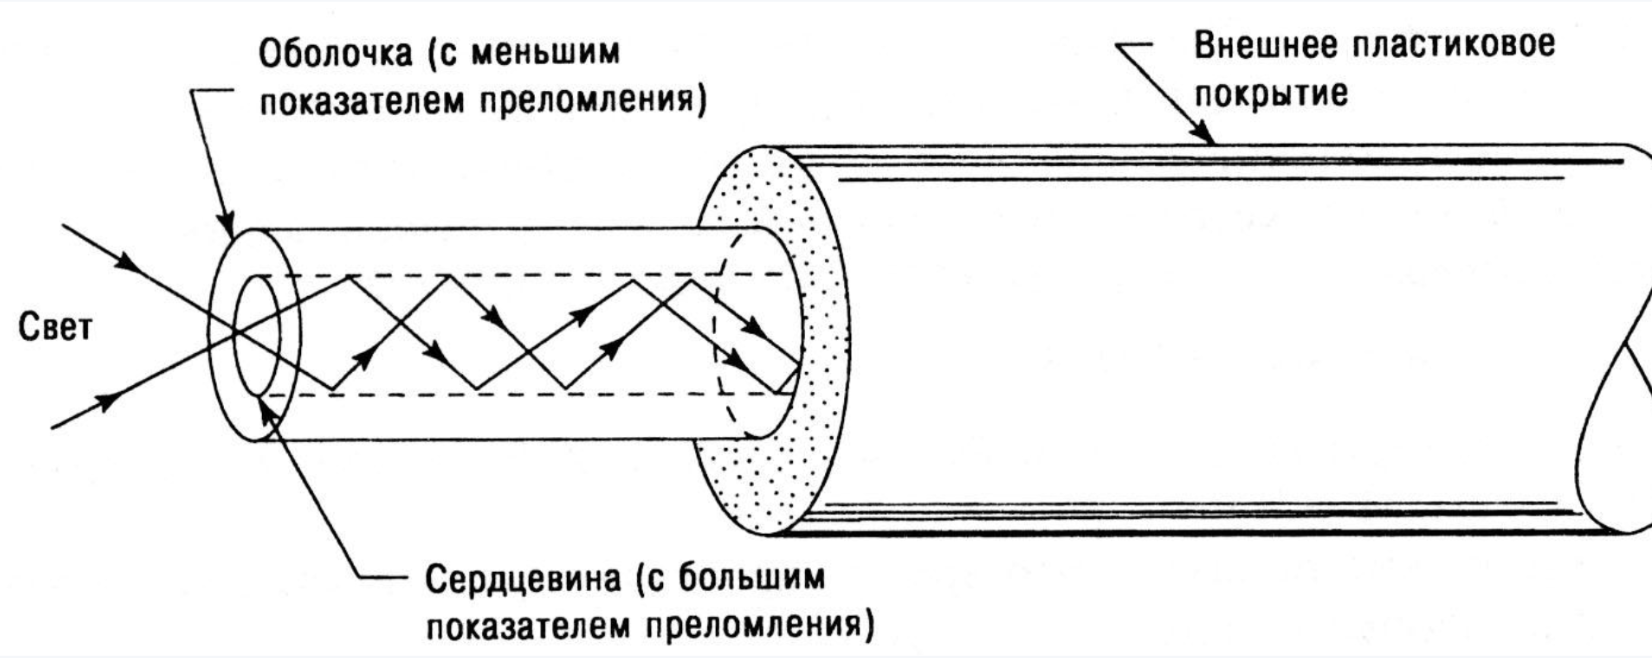
\includegraphics[width=0.7\textwidth]{pictures/fiber_structure.png}
\caption{Структура оптического волокна с сердцевиной и оболочкой}
\label{fig:fiber_structure}
\end{figure}

Принцип передачи информации по оптоволокну основан на явлении полного внутреннего отражения. Это физическое явление возникает на границе раздела двух сред с разными показателями преломления при условии, что угол падения луча превышает критический угол:
\begin{equation}
    \theta_{кр} = \arcsin\left(\frac{n_2}{n_1}\right)
\end{equation}

где $n_1$ — показатель преломления сердцевины, $n_2$ — показатель преломления оболочки.
При полном внутреннем отражении вся энергия падающей волны отражается обратно в оптически более плотную среду. Это позволяет передавать свет на большие расстояния с минимальными потерями. Стоит отметить, что в соответствии с волновой теорией, даже при полном внутреннем отражении небольшая часть энергии проникает в оболочку в виде затухающего (эванесцентного) поля, глубина проникновения которого составляет порядок длины волны света.

\subsubsection{Числовая апертура оптического волокна}
Важной характеристикой оптического волокна, определяющей его способность собирать свет, является числовая апертура (NA). Она определяет максимальный угол, под которым свет, падающий на торец волокна, будет захвачен и сможет распространяться по нему за счет полного внутреннего отражения.

Рассмотрим луч света, входящий в торец волокна из среды с показателем преломления $n_0$ (обычно воздух, $n_0 \approx 1$) под углом $\alpha_{max}$ к оси волокна (Рис. \ref{fig:numerical_aperture_derivation}). Внутри сердцевины с показателем преломления $n_1$ этот луч распространяется под углом $\theta$ к оси.

\begin{figure}[H]
    \centering
    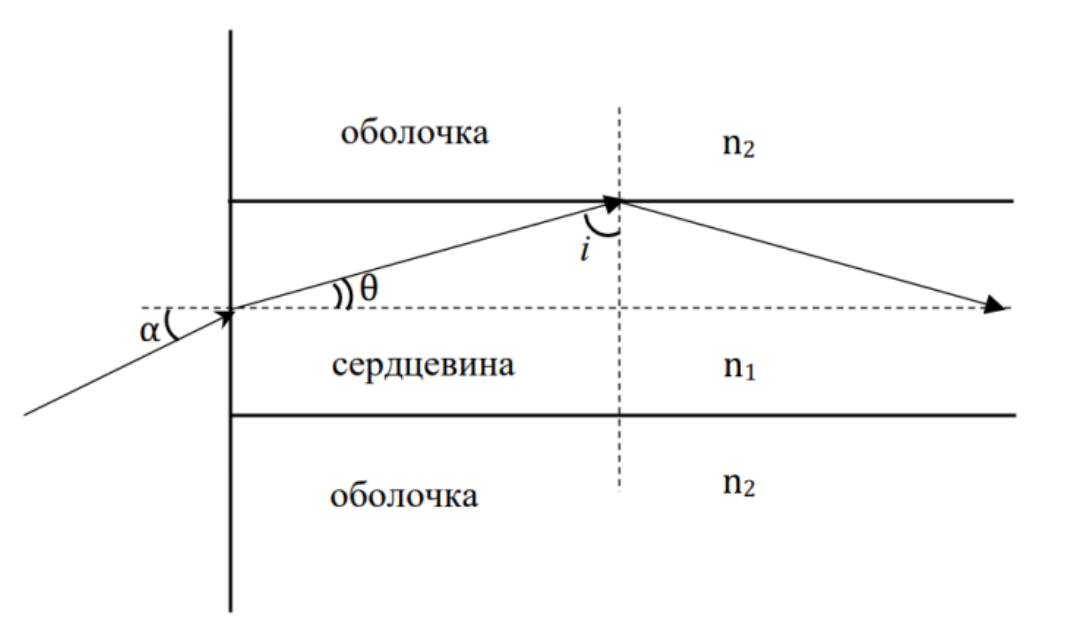
\includegraphics[width=0.7\textwidth]{pictures/numerical_aperture_derivation.png}
    \caption{Вход луча света в оптическое волокно (к выводу числовой апертуры)}
    \label{fig:numerical_aperture_derivation}
\end{figure}

На границе воздух-сердцевина по закону Снеллиуса:
\begin{equation}
    n_0 \sin\alpha_{max} = n_1 \sin\theta
\end{equation}
Для того чтобы свет распространялся по волокну, на границе сердцевина-оболочка (с показателем преломления $n_2 < n_1$) должно выполняться условие полного внутреннего отражения. Предельный случай соответствует падению луча на границу сердцевина-оболочка под критическим углом $i_{пред}$, при котором угол преломления в оболочку равен $90^\circ$. При этом угол $i$ (угол падения на границу сердцевина-оболочка) связан с углом $\theta$ соотношением $\theta + i = 90^\circ$, следовательно $\sin\theta = \cos i$.
Для максимального угла ввода $\alpha_{max}$, угол падения $i$ на границе сердцевина-оболочка должен быть не меньше предельного угла полного внутреннего отражения $i_{пред}$, для которого:
\begin{equation}
    n_1 \sin i_{пред} = n_2 \sin 90^\circ = n_2
\end{equation}
Отсюда:
\begin{equation}
    \sin i_{пред} = \frac{n_2}{n_1}
\end{equation}
Тогда для максимального угла ввода $\alpha_{max}$ имеем $\sin\theta = \cos i_{пред}$. Используя основное тригонометрическое тождество $\cos i_{пред} = \sqrt{1 - \sin^2 i_{пред}}$, получаем:
\begin{equation}
    \sin\theta = \sqrt{1 - \left(\frac{n_2}{n_1}\right)^2} = \frac{\sqrt{n_1^2 - n_2^2}}{n_1}
\end{equation}
Подставляя это выражение для $\sin\theta$ в закон Снеллиуса для границы воздух-сердцевина:
\begin{equation}
    n_0 \sin\alpha_{max} = n_1 \cdot \frac{\sqrt{n_1^2 - n_2^2}}{n_1} = \sqrt{n_1^2 - n_2^2}
\end{equation}
Величина $n_0 \sin\alpha_{max}$ и называется числовой апертурой (NA) оптического волокна:
\begin{equation}
    NA = n_0 \sin\alpha_{max} = \sqrt{n_1^2 - n_2^2}
    \label{eq:numerical_aperture}
\end{equation}
Для случая, когда свет вводится из воздуха ($n_0 \approx 1$), формула упрощается:
\begin{equation}
    NA = \sin\alpha_{max} = \sqrt{n_1^2 - n_2^2}
\end{equation}
Числовая апертура зависит только от показателей преломления сердцевины и оболочки. Как правило, разница показателей преломления $\Delta n = n_1 - n_2$ мала, порядка $10^{-3} - 10^{-2}$. В этом случае можно использовать приближенное выражение:
\begin{equation}
    NA = \sqrt{(n_1 - n_2)(n_1 + n_2)} \approx \sqrt{2n_1\Delta n} \approx \sqrt{2n\Delta n}
\end{equation}
где $n$ - средний показатель преломления (например, показатель преломления кварцевого стекла $n \sim 1.46$).
Числовая апертура характеризует светособирающую способность волокна: чем больше NA, тем больший угол ввода света допустим для его эффективного распространения.

\subsubsection{Одномодовые и многомодовые оптические волокна}
Одномодовые и многомодовые оптические волокна различаются по количеству мод (типов волн), которые могут распространяться в них. С точки зрения геометрической оптики, мода — это траектория, по которой распространяется свет, и каждой моде соответствует определенный угол распространения $\theta$ (или $i$ относительно нормали к границе раздела). С точки зрения волновой оптики, каждой моде соответствует определенное устойчивое распределение электромагнитного поля внутри световода. На Рис. \ref{fig:field_distribution_first_mode} представлено распределение модуля напряженности электрического поля по сечению световода для первой (основной) моды. На Рис. \ref{fig:full_field_distribution} представлено распределение модуля напряженности электрического поля по сечению световода для всех мод.

\begin{figure}[H]
    \centering
    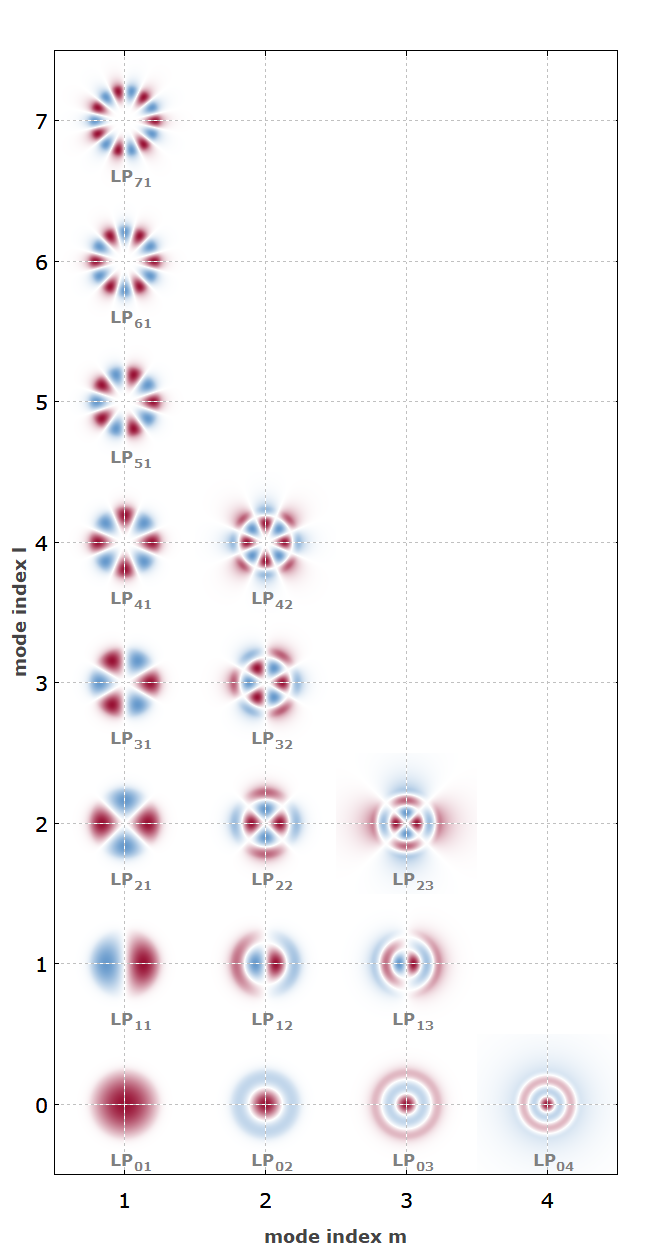
\includegraphics[width=0.75\textwidth]{pictures/full_field_distribution.png}
    \caption{Распределение электрической составляющей поля для всех мод}
    \label{fig:full_field_distribution}
\end{figure}

\begin{figure}[H]
    \centering
    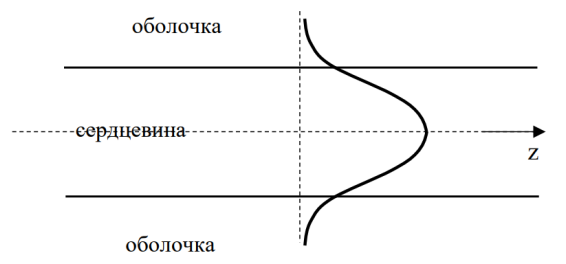
\includegraphics[width=0.7\textwidth]{pictures/field_distribution_first_mode.png}
    \caption{Распределение электрической составляющей поля для первой моды}
    \label{fig:field_distribution_first_mode}
\end{figure}

% Начало научного изложения о модах
Оптические волокна, включая используемые в телекоммуникациях, классифицируются на два основных типа: одномодовые (SMF) и многомодовые (MMF). Исторически, первые коммерчески доступные волокна характеризовались относительно большим диаметром светонесущей сердцевины, обусловленным технологическими ограничениями их производства. Такая геометрия позволяла одновременное распространение множества световых мод, что и определило их наименование — многомодовые. Для понимания сущности световой моды рассмотрим качественное объяснение этого явления.

Излучение, генерируемое лазером, обладает высокой степенью когерентности, что является необходимым условием для наблюдения интерференционных эффектов, в том числе и внутри оптического волокна. Ввод излучения в волокно, даже от лазерного источника, всегда сопряжен с некоторой конечной угловой расходимостью пучка; формирование идеально параллельного луча физически невозможно. При распространении такого когерентного излучения в сердцевине волокна происходит его многократное отражение от границы раздела сердцевина-оболочка. Взаимодействие (интерференция) падающих и отраженных когерентных волн приводит к формированию в поперечном сечении волокна устойчивого, дискретного пространственного распределения интенсивности электромагнитного поля. Эти стационарные распределения поля, возникающие в ограниченной среде волновода, размеры которого сопоставимы с длиной волны излучения, и представляют собой световые моды.

Уменьшение диаметра светонесущей сердцевины до размеров, сопоставимых с длиной волны излучения, позволяет реализовать одномодовый режим распространения, при котором в поперечном сечении формируется стоячая волна только с одной областью максимальной интенсивности (основная мода). В волокнах с диаметром сердцевины, значительно превышающим длину волны, число поддерживаемых мод велико; такие структуры иногда называют световодами и их поведение может быть частично описано в рамках геометрической (лучевой) оптики. Волокна, поддерживающие малое число мод или только одну, принято называть оптическими волноводами, и их анализ требует строгого учета волновых свойств света.

\subsubsection{Межмодовая дисперсия в многомодовых волокнах}

Несмотря на историческое первенство, многомодовые волокна обладают существенным ограничением для высокоскоростной передачи информации на большие расстояния — межмодовой дисперсией. В многомодовых волокнах со ступенчатым профилем показателя преломления различные моды распространяются под разными углами к оси волокна, проходя, таким образом, различные оптические пути (рис. \ref{fig:modes_propagation}а). Это приводит к разному времени запаздывания для разных мод, в результате чего световой импульс, изначально состоящий из множества мод, на выходе из волокна оказывается уширенным во времени. Такое уширение может привести к перекрытию соседних импульсов и, как следствие, к увеличению числа ошибок при передаче данных.

\begin{figure}[H]
    \centering
    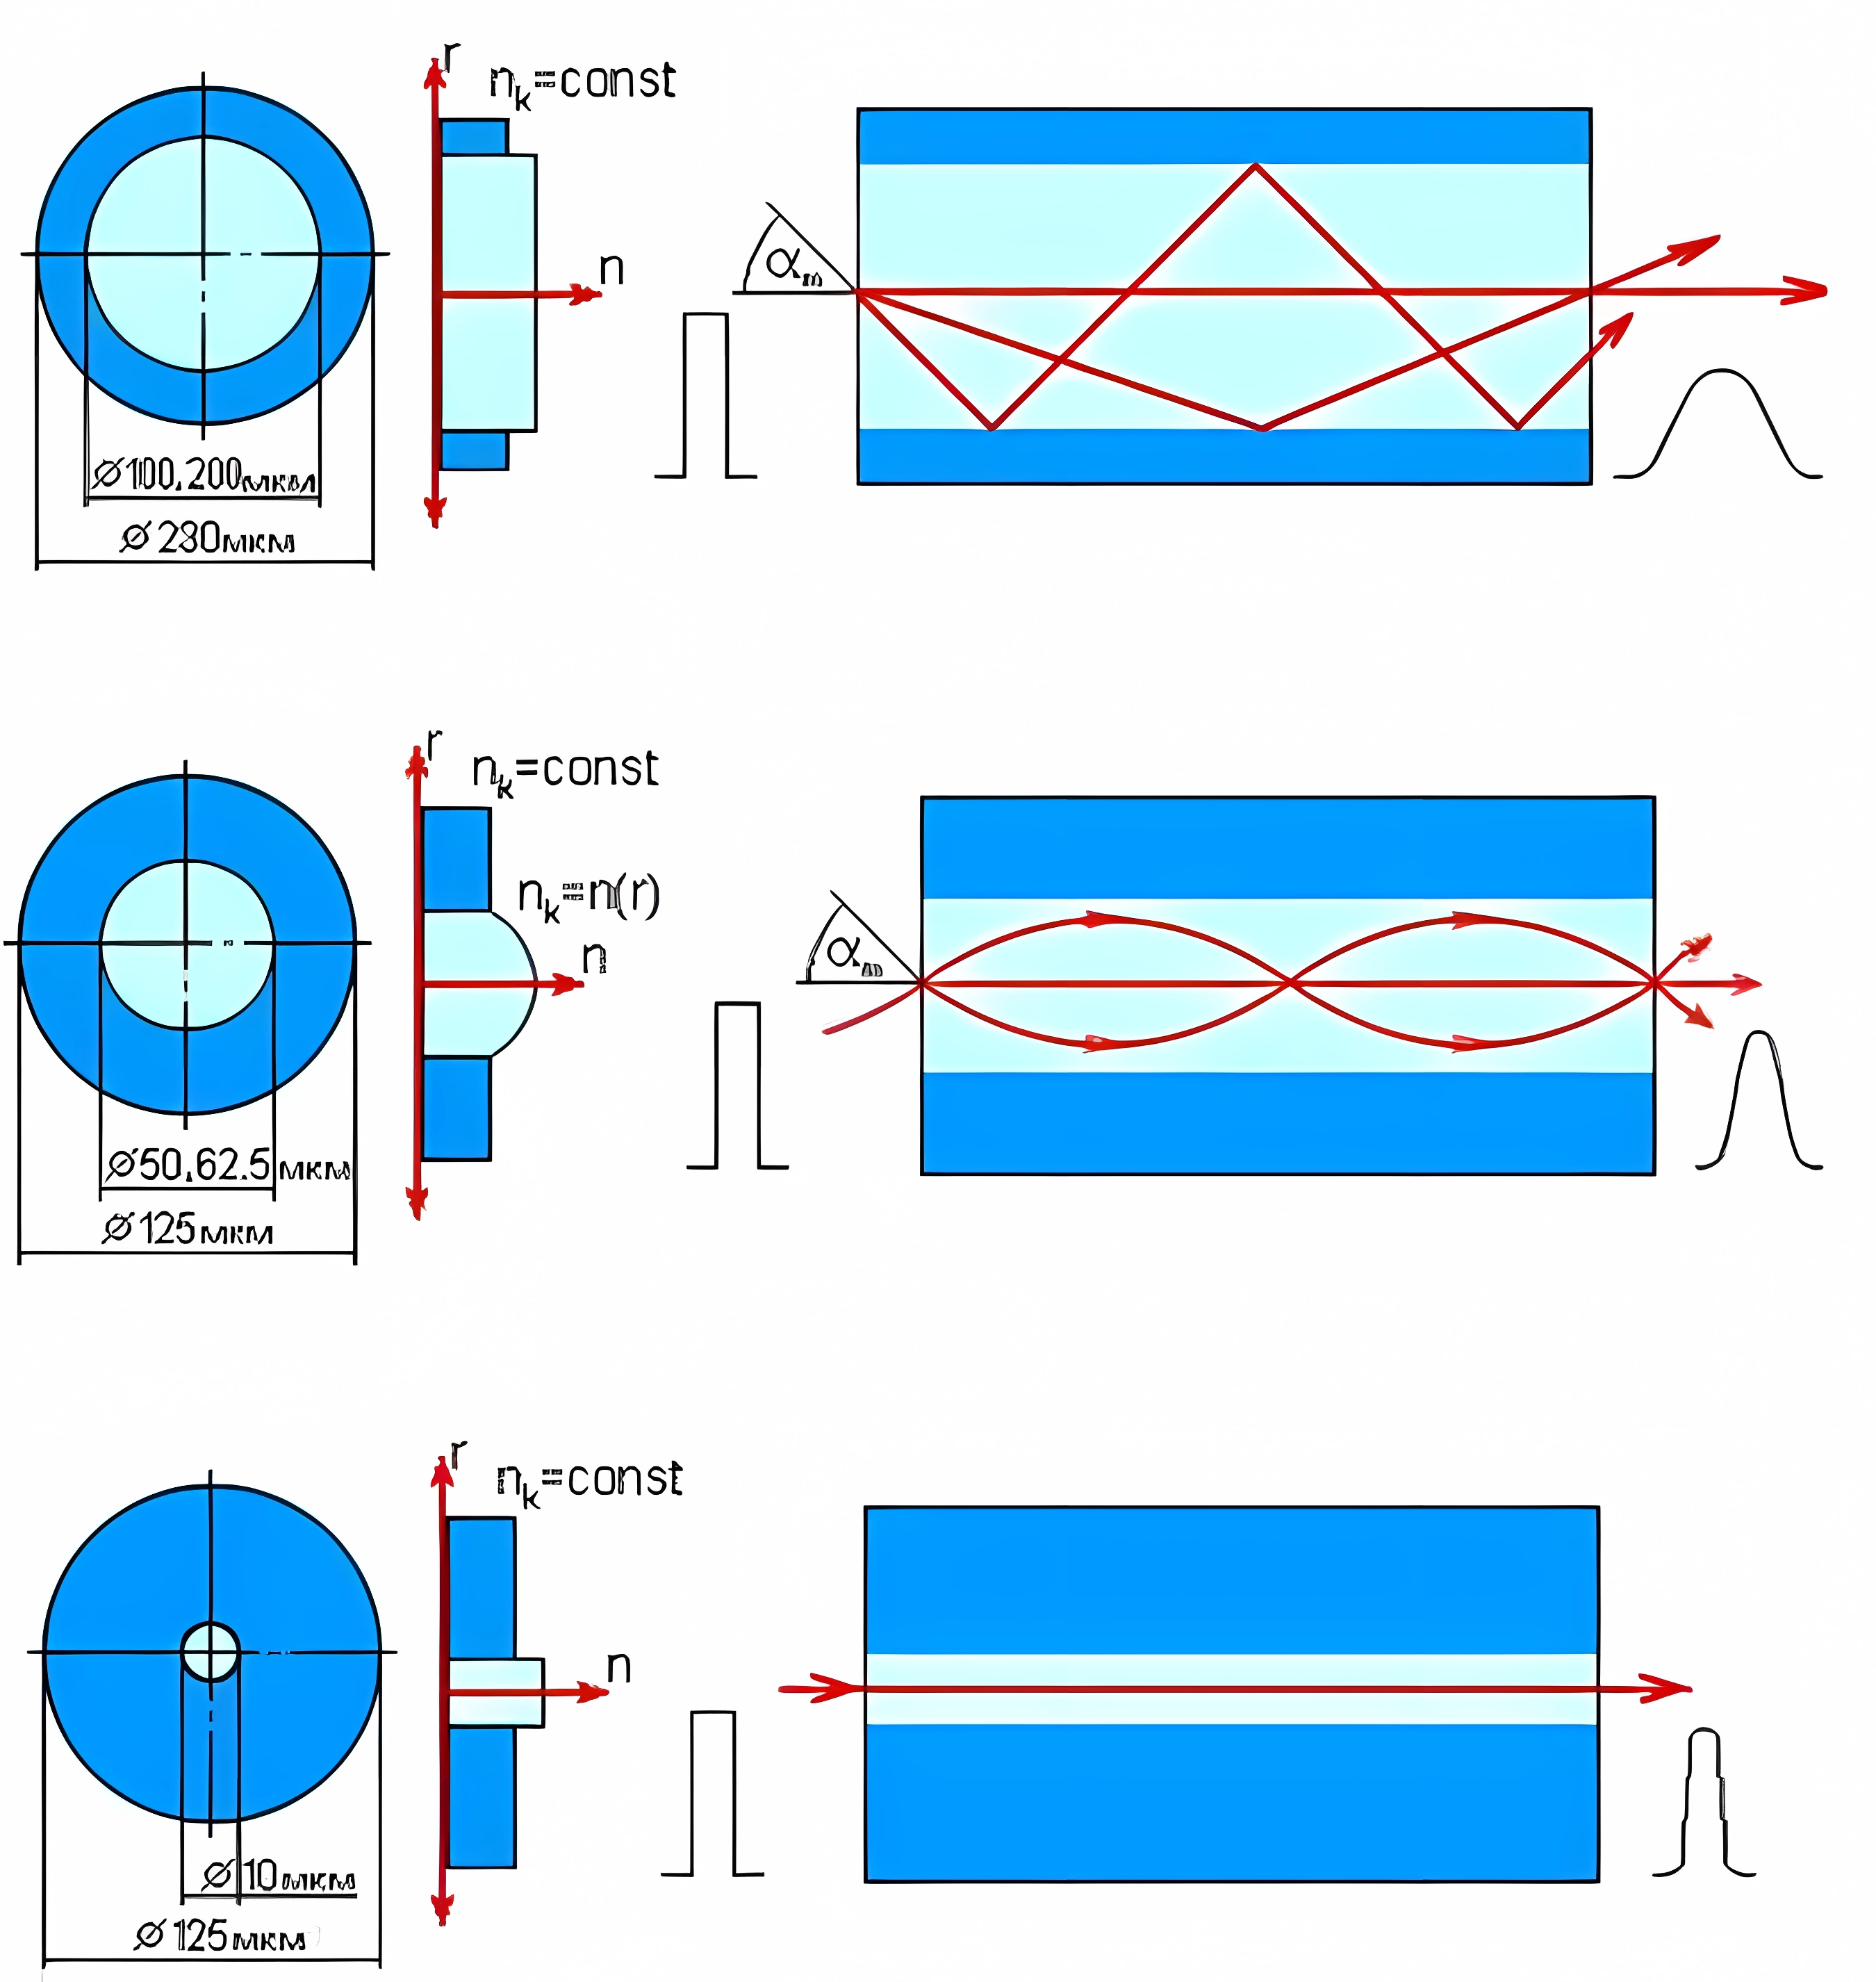
\includegraphics[width=0.7\textwidth]{pictures/modes_propagation.png}
    \caption{Распространение светового импульса в волокнах с различными профилями показателя преломления. Сверху-вниз: ступенчатый многомодовый, градиентный многомодовый, одномодовый}
    \label{fig:modes_propagation}
\end{figure}

Разработка многомодовых волокон с градиентным профилем показателя преломления (рис. \ref{fig:modes_propagation}б) позволила частично компенсировать межмодовую дисперсию за счет того, что моды высших порядков, распространяющиеся по более длинным траекториям, проходят участки с меньшим показателем преломления и, соответственно, с большей скоростью. Однако кардинальное решение проблемы межмодовой дисперсии было достигнуто с созданием одномодовых волокон (рис. \ref{fig:modes_propagation}в). В отсутствие других мод, явление межмодовой дисперсии в них не проявляется, что обеспечивает сохранение формы и длительности световых импульсов при их распространении.

В настоящее время в телекоммуникационных системах применяются оба типа волокон, однако одномодовые волокна получили значительно более широкое распространение, особенно в магистральных и протяженных линиях связи, благодаря их превосходным характеристикам по скорости и дальности передачи. Стоимость одномодовых волокон сопоставима со стоимостью многомодовых, что делает их предпочтительным выбором для большинства современных инсталляций.

\subsubsection{Волноводный параметр (V-параметр)}
Для строгого описания распространения света в оптическом волокне необходимо решать волновое уравнение, получаемое из уравнений Максвелла, с учетом геометрии волокна (цилиндрическая сердцевина и оболочка) и соответствующих граничных условий на границе раздела сердцевина-оболочка. Эти граничные условия требуют непрерывности тангенциальных компонент электрического и магнитного полей.

Решение волнового уравнения для цилиндрического диэлектрического волновода приводит к набору дискретных решений, каждое из которых соответствует определенной моде. В процессе решения, обычно методом разделения переменных в цилиндрических координатах, возникают функции Бесселя для описания поля в сердцевине и модифицированные функции Бесселя (функции Ханкеля) для описания поля в оболочке.

Применение граничных условий приводит к так называемому характеристическому (или дисперсионному) уравнению. Именно при анализе и нормировке этого характеристического уравнения естественным образом возникает безразмерная величина, называемая нормированной частотой или V-параметром:
\begin{equation}
    V = \frac{2\pi a}{\lambda} \sqrt{n_1^2 - n_2^2} = \frac{2\pi a}{\lambda} \cdot NA
    % \label{eq:V_parameter_definition_origin} % Метка уже есть выше, если это расширение
\end{equation}
где $a$ — радиус сердцевины волокна, $\lambda$ — длина волны света в вакууме, $NA = \sqrt{n_1^2 - n_2^2}$ — числовая апертура волокна.

Корни характеристического уравнения, а следовательно, и количество поддерживаемых мод, напрямую зависят от значения V-параметра. Именно поэтому условие одномодового режима ($V < 2.405$) и оценка количества мод в многомодовом волокне ($N \approx V^2/2$) выражаются через этот параметр.

\subsubsection{Волоконно-оптические датчики на основе структуры SMS}
Структуры типа SMS (SingleMode-MultiMode-SingleMode), состоящие из последовательно соединенных отрезков одномодового (SMF), многомодового (MMF) и снова одномодового волокна, представляют значительный интерес для создания волоконно-оптических датчиков. Их высокая чувствительность к внешним воздействиям, таким как механическая деформация, температура и показатель преломления окружающей среды, обусловлена эффектом межмодовой интерференции (MMI) в многомодовом участке.

\begin{figure}[H]
    \centering
    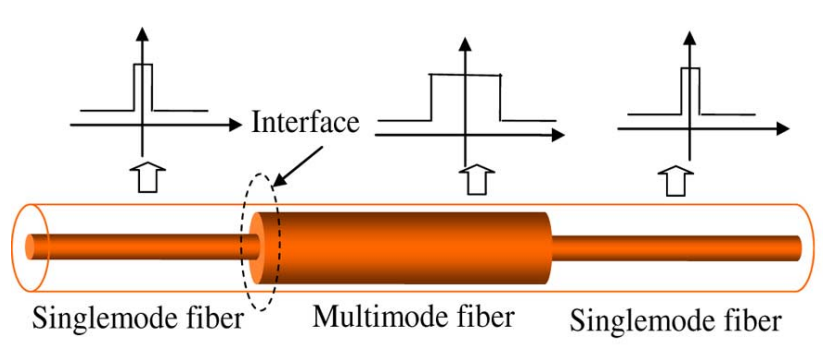
\includegraphics[width=0.8\textwidth]{pictures/sms_sensor_principle.png} % Убедитесь, что файл изображения доступен по этому пути
    \caption{Схематическое изображение структуры SMS и принцип распространения света. На входе в MMF основная мода SMF возбуждает несколько мод в MMF.}
    \label{fig:sms_sensor_principle}
\end{figure}

Принцип действия SMS-датчика основан на межмодовой интерференции (MMI) в многомодовом участке волокна (MMF), расположенном между двумя одномодовыми волокнами (SMF). Излучение из входного SMF возбуждает в MMF несколько мод, каждая из которых распространяется со своей характерной фазовой скоростью. Это приводит к накоплению зависящей от длины волны ($\lambda$) разности фаз между модами по мере их прохождения по участку MMF длиной $L_{MMF}$. На выходе MMF происходит суперпозиция этих мод. Эффективность связи результирующего интерференционного поля с основной модой выходного SMF определяет спектр пропускания всей структуры. Поскольку условия интерференции, а следовательно и коэффициенты связи, зависят от $\lambda$ (через фазовые скорости мод и накопленные фазы), спектр пропускания характеризуется чередующимися максимумами и минимумами (провалами). Провалы возникают на тех длинах волн, где преимущественно деструктивная интерференция минимизирует передачу света в выходное SMF.

Чувствительность SMS-структур к внешним воздействиям, таким как продольное растяжение, является ключевой для их применения в качестве датчиков. При растяжении изменяется как физическая длина $L_{MMF}$, так и, вследствие упругооптического эффекта, показатель преломления материала MMF (в частности, сердцевины $n_{co}$). Оба эти изменения модифицируют условия MMI и вызывают сдвиг спектральных характеристик (положения максимумов и минимумов). Для деформаций установлено, что относительный сдвиг длины волны $\Delta\lambda/\lambda_0$ некоторого спектрального признака (например, минимума) пропорционален относительному изменению длины многомодового участка $\Delta L_{MMF}/L_{MMF,0}$:
\begin{equation}
    \frac{\Delta\lambda}{\lambda_0} \approx \frac{\Delta L_{MMF}}{L_{MMF,0}}
    \label{eq:sms_sensitivity}
\end{equation}
Регистрация величины этого сдвига $\Delta\lambda$ позволяет точно определить степень деформации $\Delta L_{MMF}$. Таким образом, SMS-структуры функционируют как компактные волоконные интерферометры, эффективно преобразующие изменения физических параметров (таких как длина или показатель преломления) в измеряемые сдвиги спектральных характеристик, что делает их перспективными для детектирования деформаций, температуры и других физических величин.

\subsubsection{Спекл-картины в многомодовых волокнах и их применение}
\label{sec:speckles}
Спекл-структуры, или спекл-картины, представляют собой гранулированные интерференционные узоры, возникающие при распространении когерентного излучения в среде с оптическими неоднородностями или при его отражении/пропускании через диффузно-рассеивающие объекты. В контексте волоконной оптики, такими «диффузорами» могут выступать микронеровности и случайные флуктуации показателя преломления сердцевины и оболочки, существующие в пределах допусков на изготовление оптического волокна, особенно многомодового.

\begin{figure}[H]
    \centering
    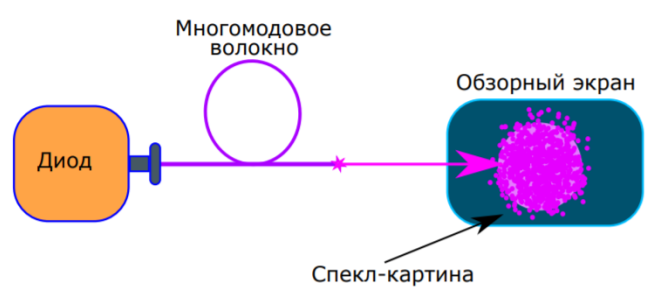
\includegraphics[width=0.8\textwidth]{pictures/speckle_pattern_scheme.png}
    \caption{Схема для наблюдения спекл-картины}
    \label{fig:speckle_pattern}
\end{figure}


Причина формирования спекл-картин при прохождении когерентного света через многомодовые волоконные световоды (MMF) заключается в интерференции большого числа направляемых мод. Каждая из этих мод обладает сложным пространственным распределением амплитуды в поперечном сечении световода и, после прохождения некоторого расстояния, практически случайной фазой относительно других мод. Эта случайность фаз обусловлена несколькими факторами: различиями в оптических путях для разных мод (модовая дисперсия), неизбежными микроизгибами волокна, внутренними напряжениями и структурными несовершенствами материала, а также процессами перераспределения энергии между модами (модовое смешение или связь мод). В результате суперпозиции этих многочисленных когерентных, но случайно-сфазированных волн на выходе MMF и формируется сложная, но стационарная во времени (при неизменных условиях) зернистая структура интенсивностей — спекл-картина.

Уникальность и высокая чувствительность спекл-картины к малейшим изменениям состояния MMF делают ее ценным носителем измерительной информации. Благодаря своей высокой чувствительности, простоте реализации (часто требуется лишь источник когерентного света, отрезок MMF и камера для регистрации спеклов), сенсоры на основе анализа спекл-картин находят применение в высокоточных измерениях деформаций, вибраций, давления.

\subsection{Экспериментальная установка}
\label{sec:experimental_setup}
Для исследования характеристик датчика продольного растяжения на основе SMS-структуры была собрана экспериментальная установка, основные компоненты которой включают:

\textbf{Источник излучения:} В качестве источника широкополосного излучения использовался оптический тестер EXFO FOT-600, работающий в режиме источника света. Данный прибор обеспечивает стабильное излучение в требуемом для экспериментов спектральном диапазоне.

\begin{figure}[H]
    \centering
    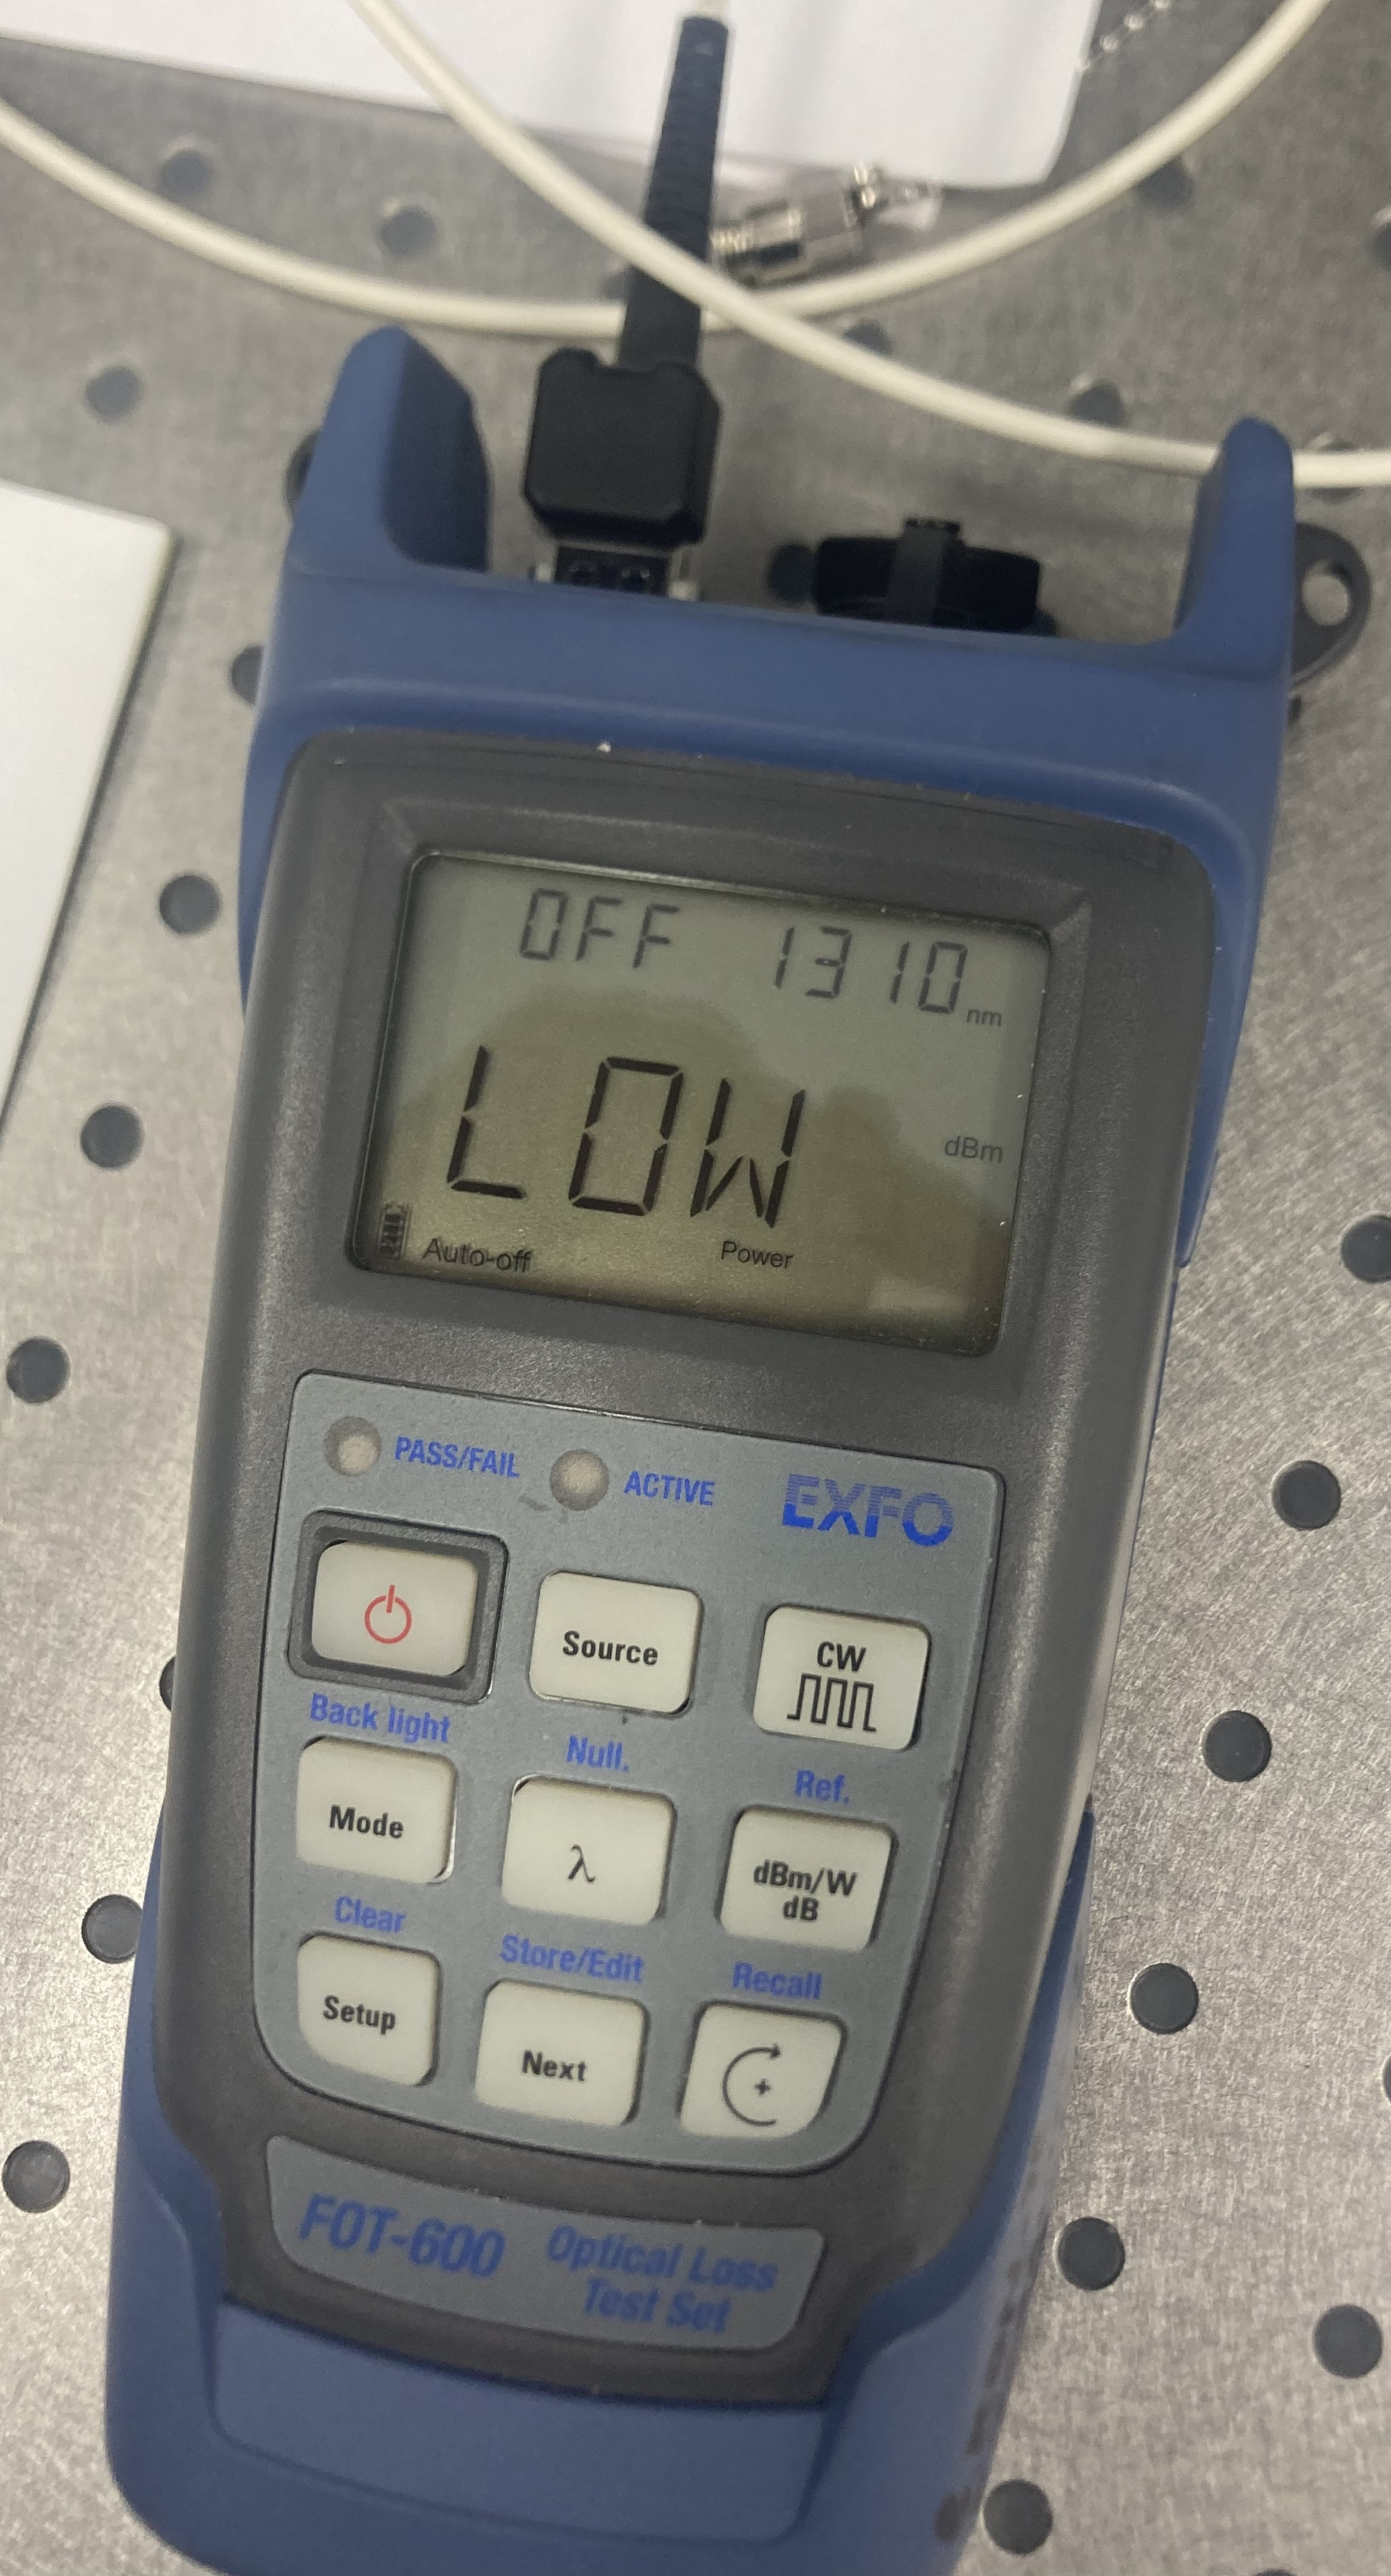
\includegraphics[width=0.5\textwidth]{pictures/exfo_fot_600.png} % Замените на актуальное имя файла
    \caption{Оптический тестер EXFO FOT-600, используемый в качестве источника излучения}
    \label{fig:exfo_fot_600}
\end{figure}

\textbf{Оптический усилитель:} Для усиления оптического сигнала перед его вводом в исследуемый датчик применялся эрбиевый волоконный усилитель (EDFA). Усиление необходимо для компенсации потерь в SMS-структуре и обеспечения достаточного уровня сигнала на входе спектроанализатора.

\begin{figure}[H]
    \centering
    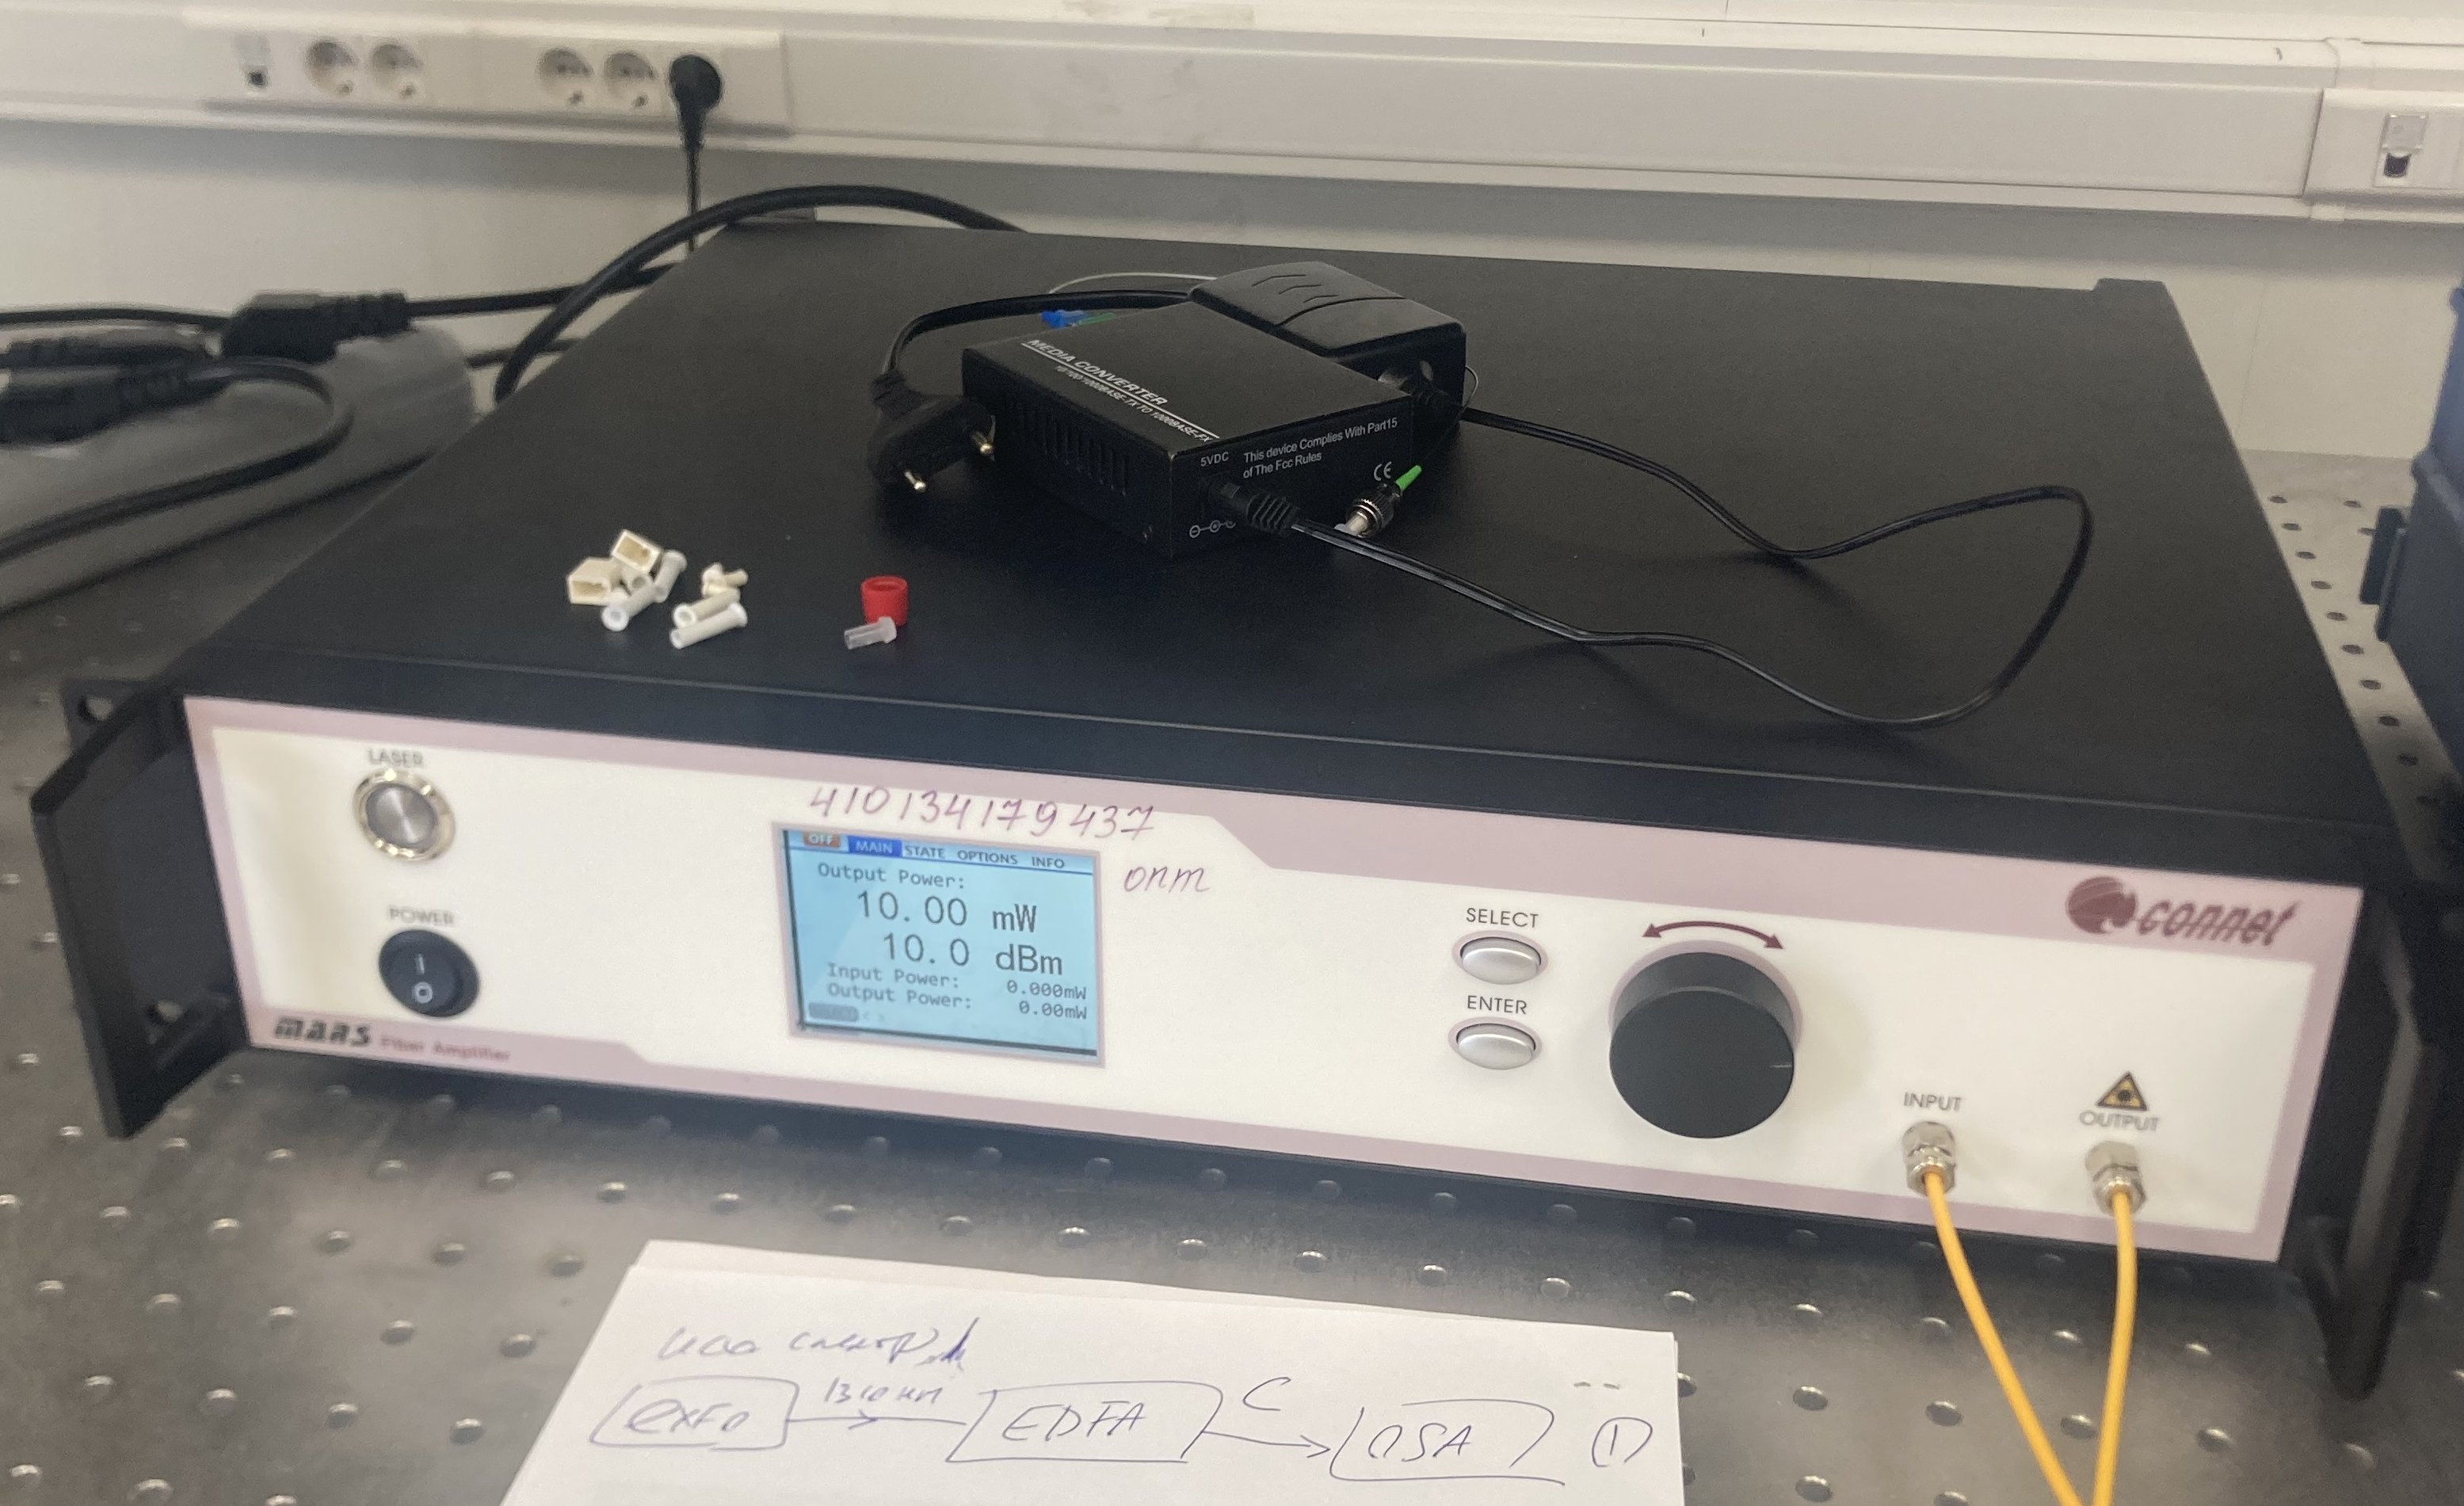
\includegraphics[width=0.7\textwidth]{pictures/edfa_amplifier.png} % Замените на актуальное имя файла
    \caption{Эрбиевый волоконный усилитель (EDFA)}
    \label{fig:edfa_amplifier}
\end{figure}

\textbf{Исследуемый датчик SMS:} Чувствительный элемент представляет собой отрезок волокна со структурой одномод-многомод-одномод (SMS). Один конец датчика был жестко закреплен, а ко второму концу прикладывалась дозированная продольная нагрузка.

\begin{figure}[H]
    \centering
    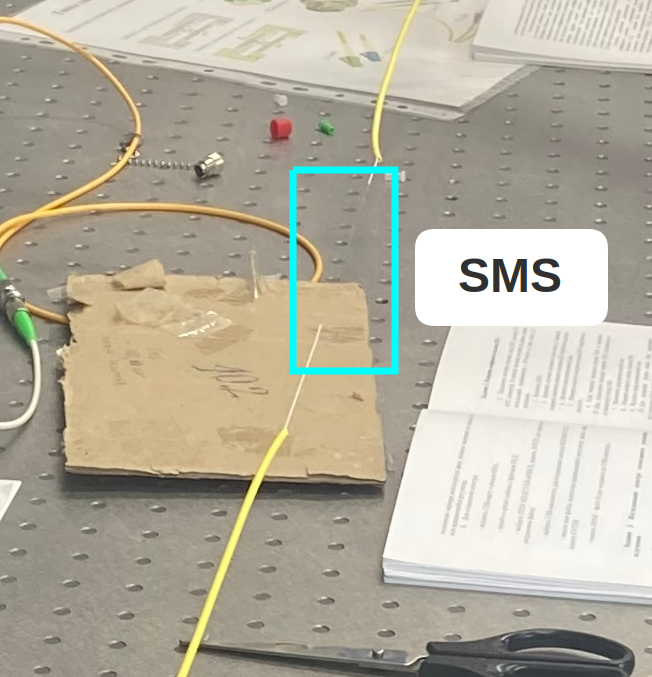
\includegraphics[width=0.5\textwidth]{pictures/sms_sensor_mounted.png} % Замените на актуальное имя файла
    \caption{Датчик на основе SMS-структуры, подготовленный для эксперимента по растяжению}
    \label{fig:sms_sensor_mounted}
\end{figure}

\textbf{Грузики:} Растяжение датчика SMS осуществлялось с помощью набора калиброванных грузиков, которые подвешивались к свободному концу волокна. Это позволяло прикладывать точно известную силу и, соответственно, вызывать контролируемую деформацию.

\begin{figure}[H]
    \centering
    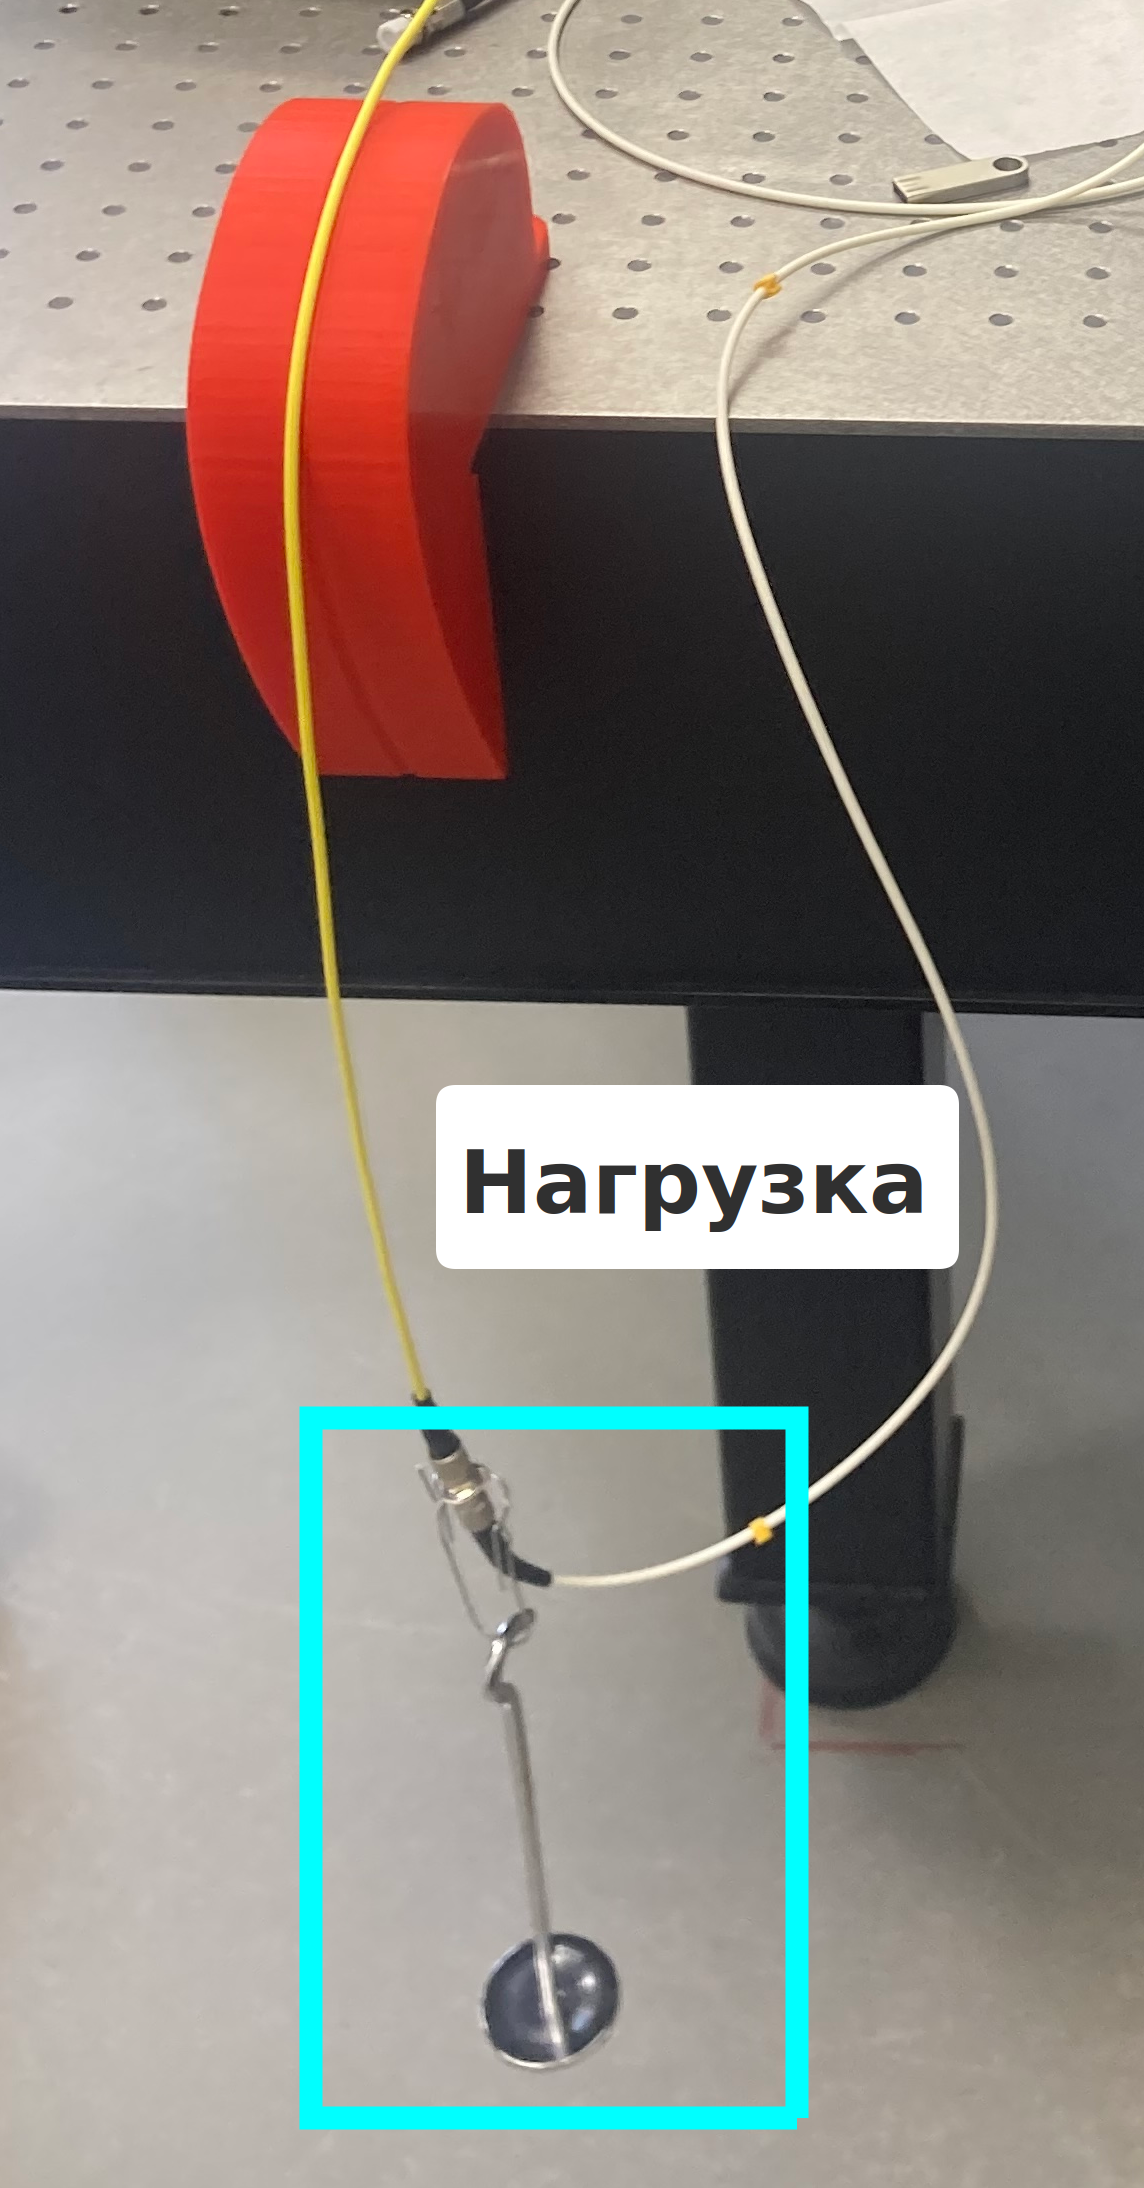
\includegraphics[width=0.5\textwidth]{pictures/calibration_weights.png} % Замените на актуальное имя файла
    \caption{Набор калиброванных грузиков для создания продольной нагрузки на датчик}
    \label{fig:calibration_weights}
\end{figure}

\textbf{Анализатор оптического спектра:} Для регистрации и анализа спектра пропускания излучения, прошедшего через SMS-датчик, использовался анализатор оптического спектра YOKOGAWA AQ6370C. Данный прибор позволяет с высоким разрешением измерять зависимость интенсивности света от длины волны.

\begin{figure}[H]
    \centering
    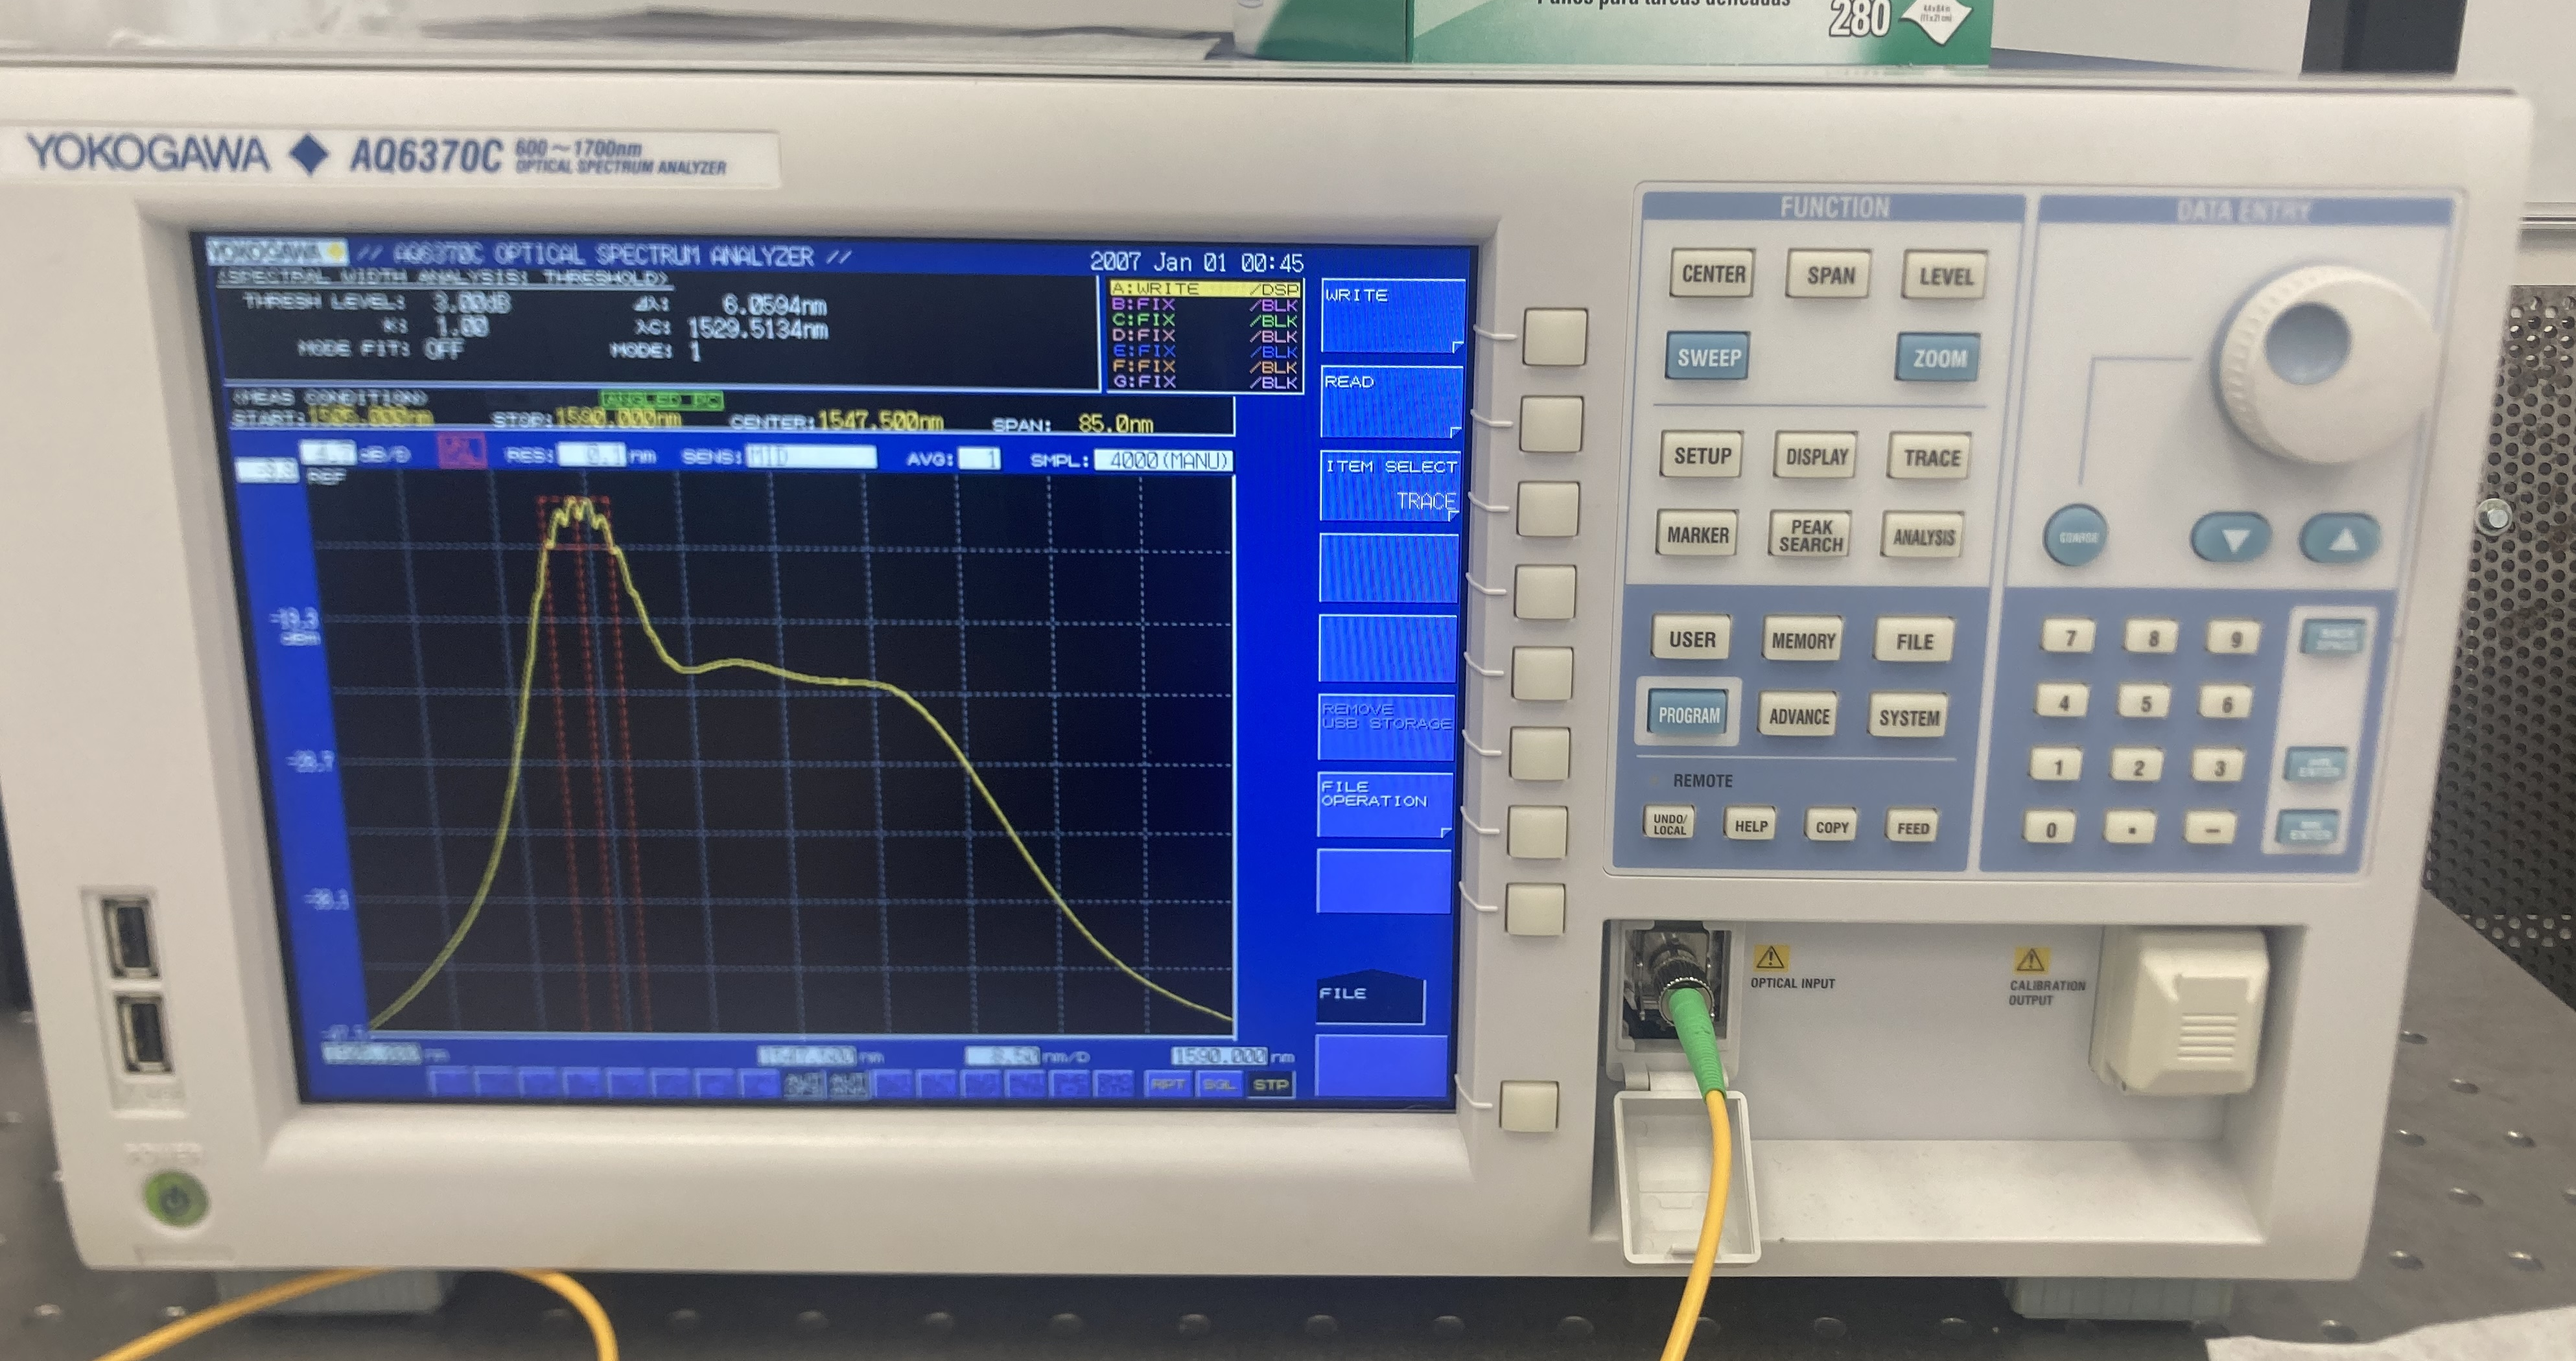
\includegraphics[width=0.7\textwidth]{pictures/yokogawa_aq6370c.png} % Замените на актуальное имя файла
    \caption{Анализатор оптического спектра YOKOGAWA AQ6370C}
    \label{fig:yokogawa_aq6370c}
\end{figure}


Излучение от тестера EXFO FOT-600 поступало на вход EDFA, усиливалось и затем вводилось в SMS-датчик. Выходной сигнал с датчика регистрировался спектроанализатором YOKOGAWA AQ6370C. В ходе эксперимента к датчику прикладывались различные нагрузки с помощью грузиков, и для каждой нагрузки снимался соответствующий спектр пропускания.

